\documentclass[a4paper]{scrreprt}

\usepackage[T1]{fontenc}
\usepackage[utf8]{inputenc}
\usepackage{graphicx}
\usepackage{svg}
\usepackage{listings}
%\usepackage{showframe}
\usepackage{fullpage}
\usepackage[colorlinks=true]{hyperref}
\usepackage{tabu}
\usepackage{float}
\usepackage{afterpage}
\usepackage{pdflscape}
\usepackage{pdfpages}

\lstdefinelanguage[ARM]{Assembly}     % add a "x64" dialect of Assemblers
   [x86masm]{Assembler} % based on the "x86masm" dialect
   % with these extra keywords:
   {
   morekeywords={MOV, LDR},
    morekeywords=[2]{.align,.cpu,.thumb,.syntax,.word},%
    alsoletter={.,0,1,2,3,4,5,6,7,8,9},%
    alsodigit={?},%
    sensitive=false,%
    morestring=[b]",%
    morecomment=[s]{/*}{*/},%
    morecomment=[l]@,%
    morecomment=[l]//,%
   }[keywords,comments,strings]
\lstset{language=[ARM]Assembly}

\title{\vspace*{60mm}Introduction to Microcontrollers Notes}
\author{James Gowans}

\begin{document}
  \maketitle

  \vspace{\fill}
\section*{Licence}
This work is licensed under the Creative Commons Attribution-ShareAlike 3.0 Unported License. To view a copy of this license, visit http://creativecommons.org/licenses/by-sa/3.0/ or send a letter to Creative Commons, 444 Castro Street, Suite 900, Mountain View, California, 94041, USA.


\newpage
\tableofcontents
\newpage
%\section{A History of Processing}
In 1971 the dawn of a new era began. Intel had just announced that they had developed ``a programmable computer on a chip.'' The chip, known as the 4004 was the first general purpose microprocessor on one silicon chip, and contained around 2300 transistors. In order to produce this chip, the layout of the transistors was hand-drawn using coloured pencils at 500 times scale. The CPU had the ability to transfer 4 bits per clock cycle, had a 12-bit address space and an 8-bit instruction. In total, it has 16 instructions which it could execute. It was used in a calculator which had an optional square root function. The calculator run around 100K instructions per second, had 1 KB of ROM and 80 bytes of RAM. 

The next year, in 1972 Intel released the 8008, an 8-bit microprocessor. The 8008 had a 14 bit address space. The first use for the 8008 was a programmable scientific calculator. In 1973 the 8008 was used as the CPU for a French desktop computer. Some consider this to be the first desktop computer. The 8008 evolved into the 8080. 

While desktop computers do take a large share of the microprocessor market, many times more microprocessors go into microcontrollers for the purpose of embedded control applications. In 1996, 25 years after the advent of the first microprocessor, 70\% of all semiconductors are used for microcontroller-based circuits. 

A processor with IO an memory is a microcontroller. In 1995, 50\% of microcontrollers manufacturered were 4-bit. 

\chapter{System Overview}

\begin{figure}[t]
  \centering
  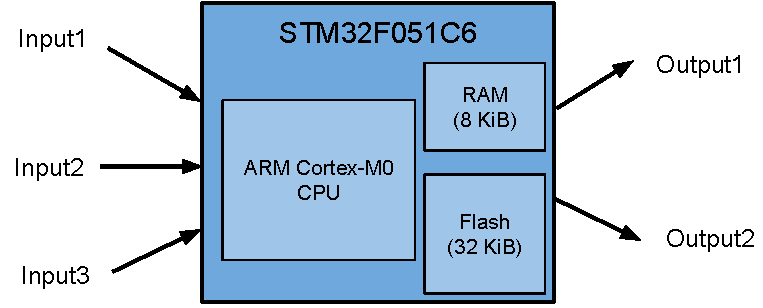
\includegraphics[width=\textwidth]{./week1/programmers_model_v0.pdf}
  \caption{The most simplified view of the internals of the STM32F051}
  \label{fig:prog_mod_v0}
\end{figure}

\section{What is a Microcontroller?}
The microcontroller can be understood by comparing it to something you are already very familiar with: the computer. Both a microcontroller and a computer can be modeled as a black box which takes in data and instructions, performs processing, and provides output.
In order to do this, a micro has some of the same internals as a computer, shown graphically in \autoref{fig:prog_mod_v0} and discussed now:
\begin{itemize}
  \item CPU: The section of the microcontroller which does the processing. It executes instructions which allows it to do arithmetic and logic operations, amongst other forms of operations.
  \item  Volatile memory (RAM:) This is general purpose memory. It can be used for storing whatever you want to store in it. Typically it stores variables which are created or changed during the course of execution of a program.
  \item Non-volatile memory (Flash): This non-volatile memory is used to store any date which must not be lost when the power to the micro is removed. Typically this would include the program code and any constants or initial values of data.
  \item Ports: Interfaces for data to move in and out of the micro. This allow it to communicate with the outside world. 
\end{itemize} 
These resources are typically orders of magnitude smaller or a micro than on a conventional computer. A micro makes up for this lack of resources with a small size, low power and low cost. A comparison of the characteristics can be seen in \autoref{table:specs_comp}.
A computer is typically defined as a multi-purpose, flexible unit able to do computation. A microcontroller on the other hand typically is hard-coded to do one specific job.\\

\begin{table}
\begin{tabu}{ >{\textbf}c | c  c  c  c  c  c }
  & \textbf{CPU} & \textbf{RAM} & \textbf{Non-volatile} & \textbf{Power} & \textbf{Size/Mass} & \textbf{Cost} \\
  \hline
  \textbf{Computer} & Dual, 3 GHz & 4 GiB & 500 GB & 100 W & Large & R 3000 \\
  \textbf{Micro} & 48 MHz & 8 KiB & 32 KiB & 50 mW & Small & R 15 \\
\end{tabu}
\caption{Comparison of specs of entry level computer to STM32F051C6.}
\label{table:specs_comp}
\end{table}

The terms \textit{microcontroller} and \textit{microprocessor} are different and should not be used interchangeably. A micro\textit{processor} is an IC which is able to perform computation, but requires external memory and peripherals to function. A micro\textit{controller} has the memory and peripherals built into it, allowing it to be fully independent. Furthermore, the interface in and out of a microprocessor is mainly just an address and data bus. In a microcontroller, these busses are internal to the device. The interfaces in and out of a microcontroller are configurable to be a wide variety of communication standards. This self-contained nature and ability to deal with a wide variert of signals allows a microcontroller to (as the name suggest) be embedded in a larger system and perform control and monitoring functions.\\

The micro we will be using is the STM32F051C6. It is manufactured by ST Microelectronics, but has an ARM Cortex-M0 CPU. ARM designed the CPU (specified how the transistors connect together). ST then takes this CPU design, adds it to their design for all of the other bits of the micro (flash, RAM, ports and much much more) and then produces the chip.

\subsection{Development board block diagram}
The development board consists of modules which connect to the microcontroller. Most of these modules are optional in that they are not required for the microcontroller to run. We will develop code later in the course to interface with some of these modules. Those which are not optional are the voltage regulator and the debugger.
Following is a brief discussion of the purpose of each of the dev board modules (peripherals).

\begin{figure}
  \centering
  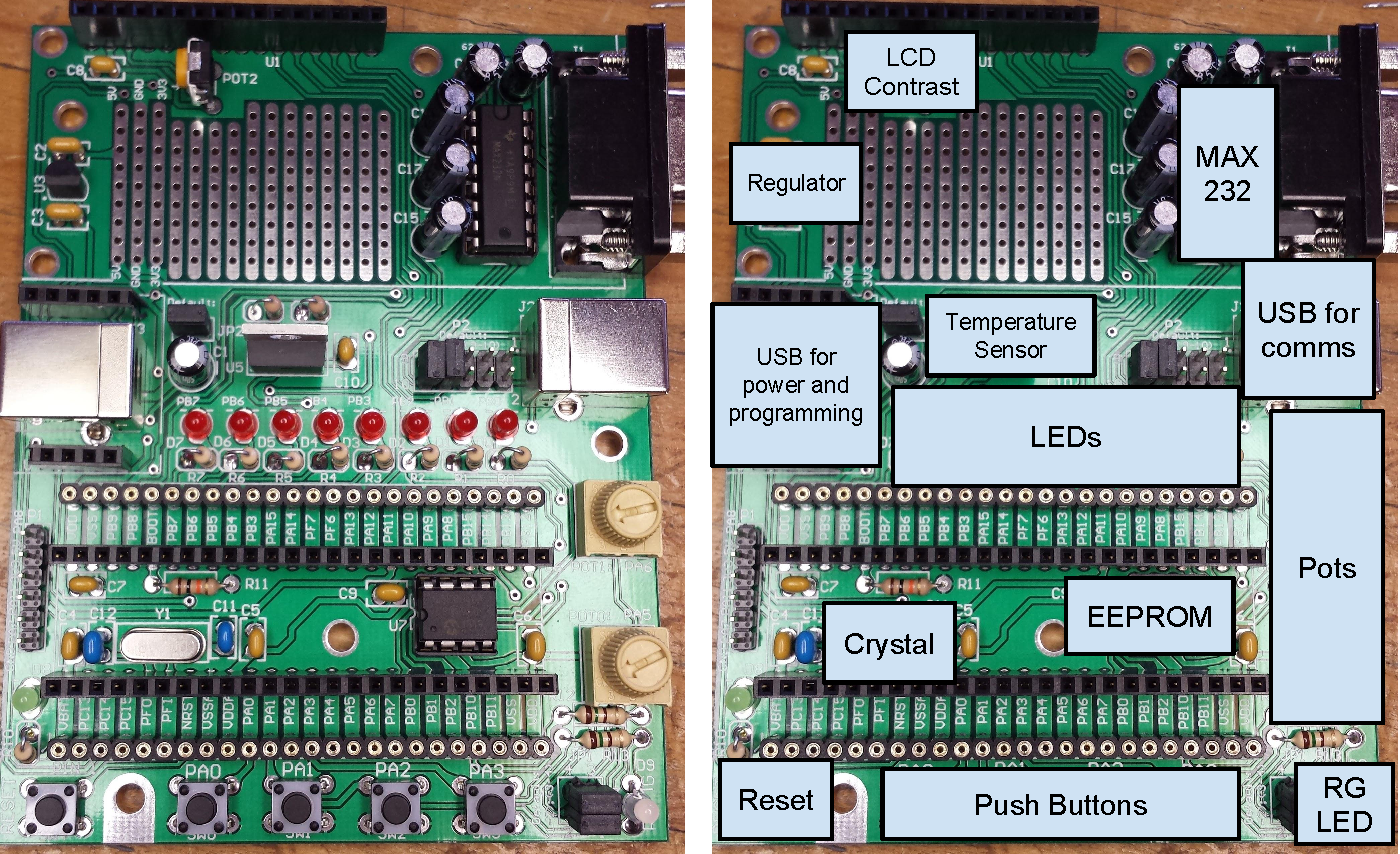
\includegraphics[width=\textwidth]{./week1/dev_board_unplugged.pdf}\\
  \vspace{3mm}
  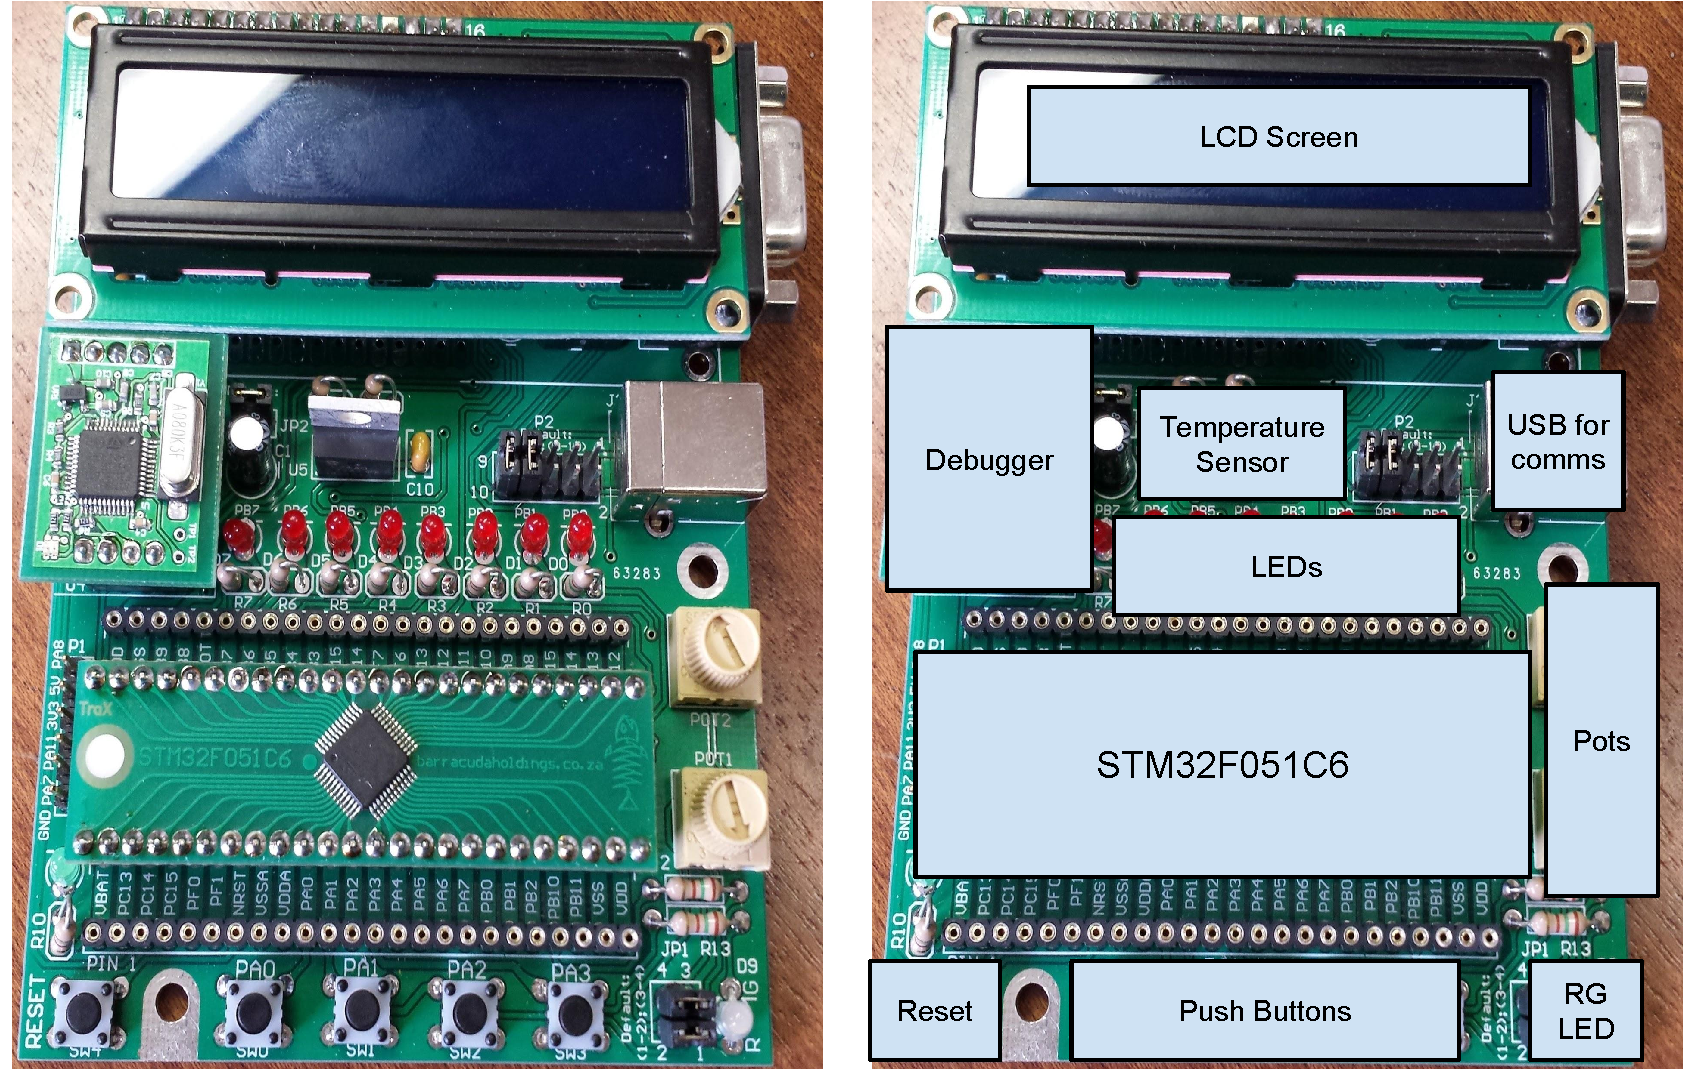
\includegraphics[width=\textwidth]{./week1/dev_board_plugged_in.pdf}
  \caption{Modules on the dev board as seen when top boards unplugged or plugged in.}
\end{figure}

\begin{itemize}
  \item STM32F051C6: This is the target microcontroller. It is connected to everything else on the board and it is where the code which we develop will execute. 
  \item Debugger: this is essentially another microcontroller running special code on it which allows it to be able to pass information between a computer and the target microcontroller. The interface to the computer is a USB connection, and the interface to the target is a protocol called Serial Wire Debug (SWD) which is similar to JTAG. The specific type of debugger which we have is a ST-Link.
  \item Regulator: A MCP1702-33/T0 chip. This converts the 5 V provided by the USB port into 3.3 V suitable for running most of the circuitry on the board. 
  \item LEDs: One byte of LEDs, active high connected to the lower byte of port B.
  \item Push buttons: Active low push buttons connected to the lower nibble of port A.
  \item Pots: 2 x 10K (or there abouts) potentiometers connected to PA5 and PA6.
  \item LCD Screen: A 16x2 screen connected to the micro in 4-bit mode. Used to display text.
  \item LCD contrast pot: The output of this potentiometer connects to the contrast pin of the LCD screen, hence allowing contrast adjustment.
  \item MAX232: This chips translates between TTL or CMOST logic level UART traffic and bi-polar higher voltage RS-232 traffic. Used for industrial communications links.
  \item USB for comms: The header allows intercepting of the UART traffic before it gets to the MAX232 and converting it to USB traffic through a small board which plugs into that header. When this facility is not being used, the jumpers on the header should be placed to allow the UART traffic to make its way to the MAX232.
  \item Temperature sensor: A TC74-A0 $I^2C$ temperature sensor.
  \item Crystal: 8 MHz quartz oscillator with 10 pF caps for removing high frequency harmonics. 
  \item EEPROM: A 25LC640A 64Kb Electronically Erasable and Programmable Read Only Memory (EEPROM) chip which communicates over SPI.
  \item RG LED: Common cathode Red/Green LED.
\end{itemize}


The full circuit schematic for the board follows. 
For now, we will forget about all of the other modules on the dev board and consider our system to be a computer talking to a debugger talking to a target micro, as shown in \autoref{fig:debugger_to_micro}. 
This is the most basic system which must be understood to allow us to load code onto the target microcontroller.

\begin{figure}[t]
  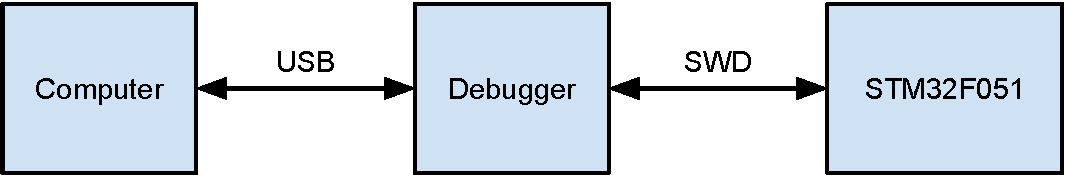
\includegraphics[width=\textwidth]{./week1/debugger_to_micro.pdf}
  \caption{Highly simpified diagram showing how micro and computer communicate}
  \label{fig:debugger_to_micro}
\end{figure}

\afterpage{
  \begin{landscape}
  %\begin{figure}
    \centering
    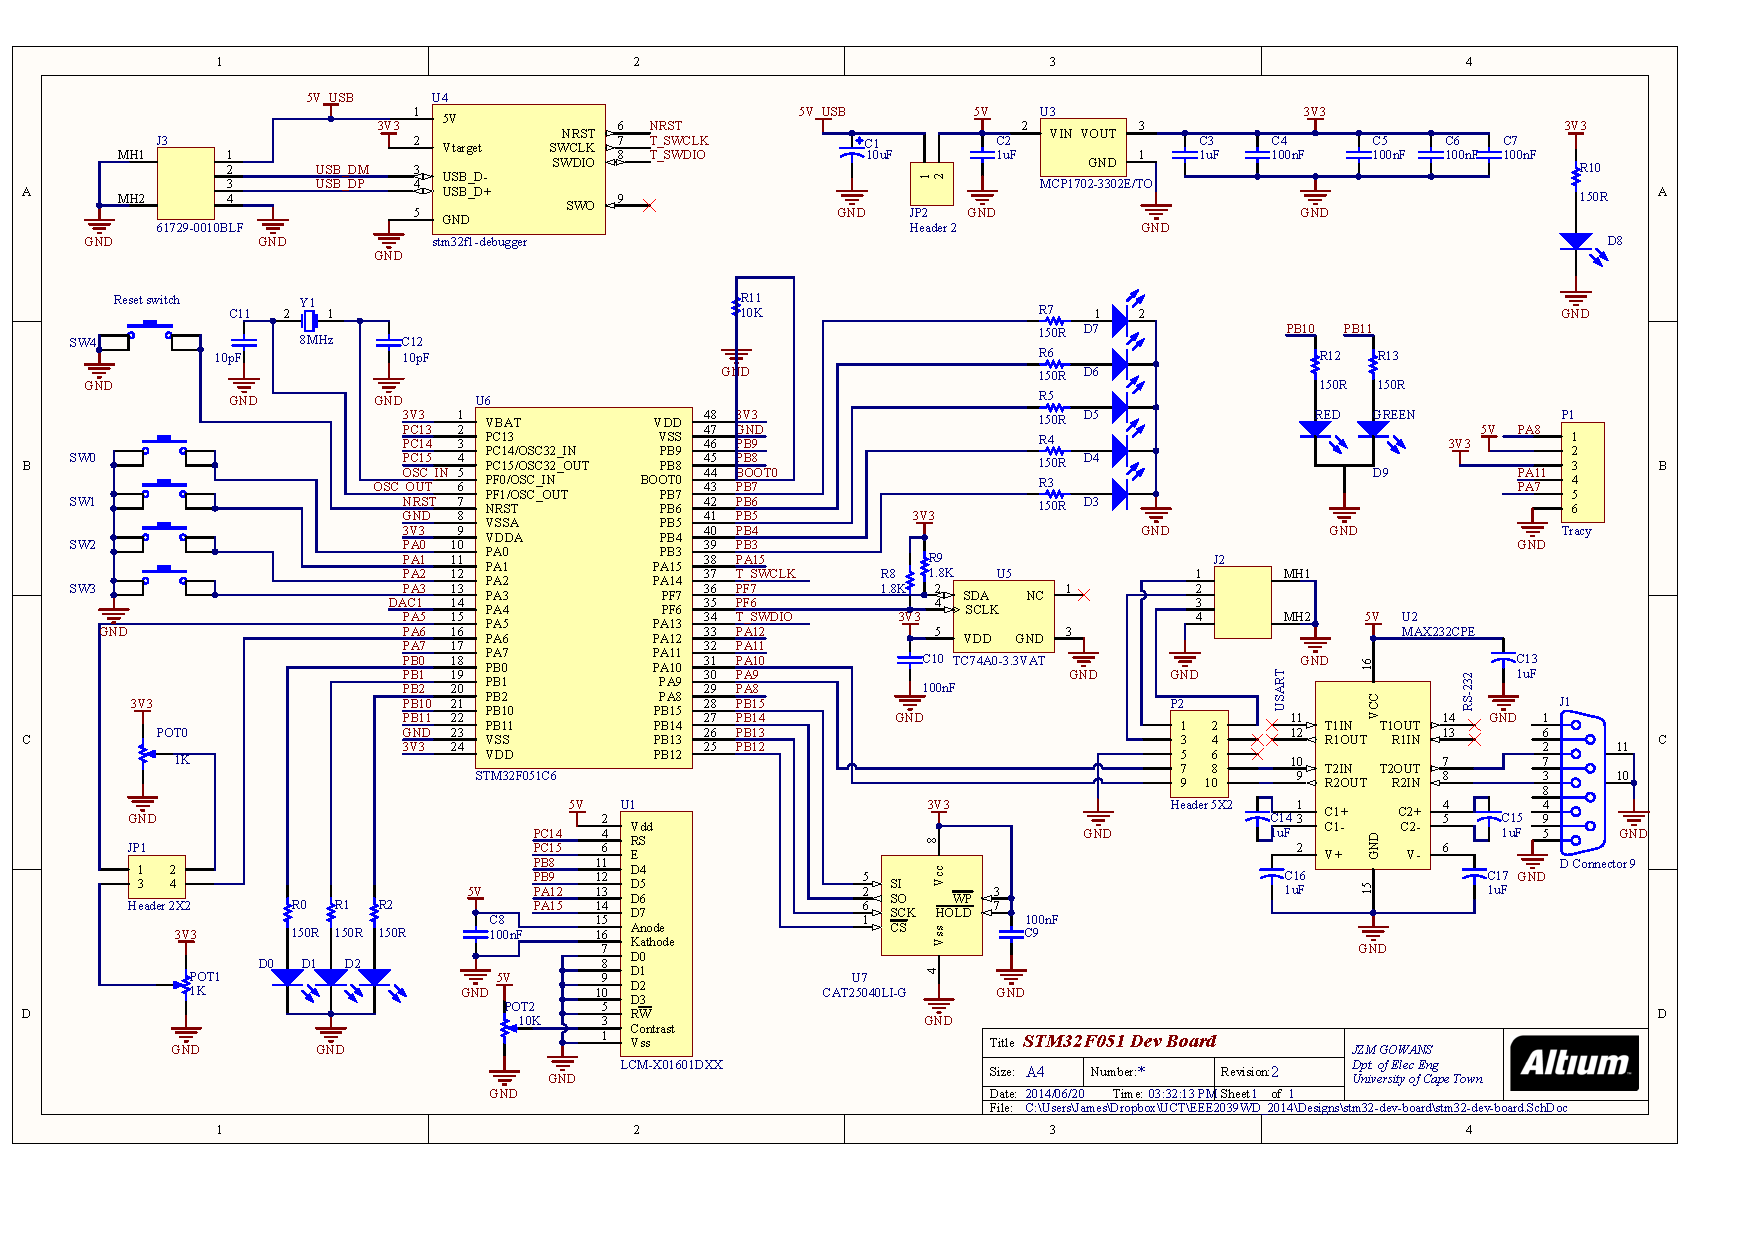
\includepdf[pages={1}, angle=90]{./week1/circuit_sch.pdf}
 % \end{figure}
 \end{landscape}
} 







%\subsection{A Short History of ARM}
%Acorn

%\chapter{Perihperals}
%Ports are typically controlled by a block of memory called perihperals. Unlike RAM which is general purpose, each register in the perihperals memory block has a specific, well defined purpose. Typically the purpose of these perihperal registes are for configuring the microcontroller to behave in a certain way or communicate with the outside world.
%These CPU registers are different to the peripheral registers mentioned earlier for the reasons that they are located inside the CPU rather than in the address space and also they are mostly general purpose: they can hold any data required in the execution of a program. 


\chapter{The ARM Cortex-M0}

At the core of a microcontroller is the CPU. Our CPU is called the Cortex-M0 and is designed by Advanced RISC Machines (ARM).
The ARM Cortex-M0 CPU is certainly the most interesting block inside the STM32F051C6. This is where all processing happens, hence this is where the instructions which we write will run. It is therefore essential that we have an intricate understanding of the CPU so that we may write useful code for it. This chapter seeks to explore the CPU in some detail.

\section{Programmer's Model of the CPU}
\begin{figure}[t]
  \centering
  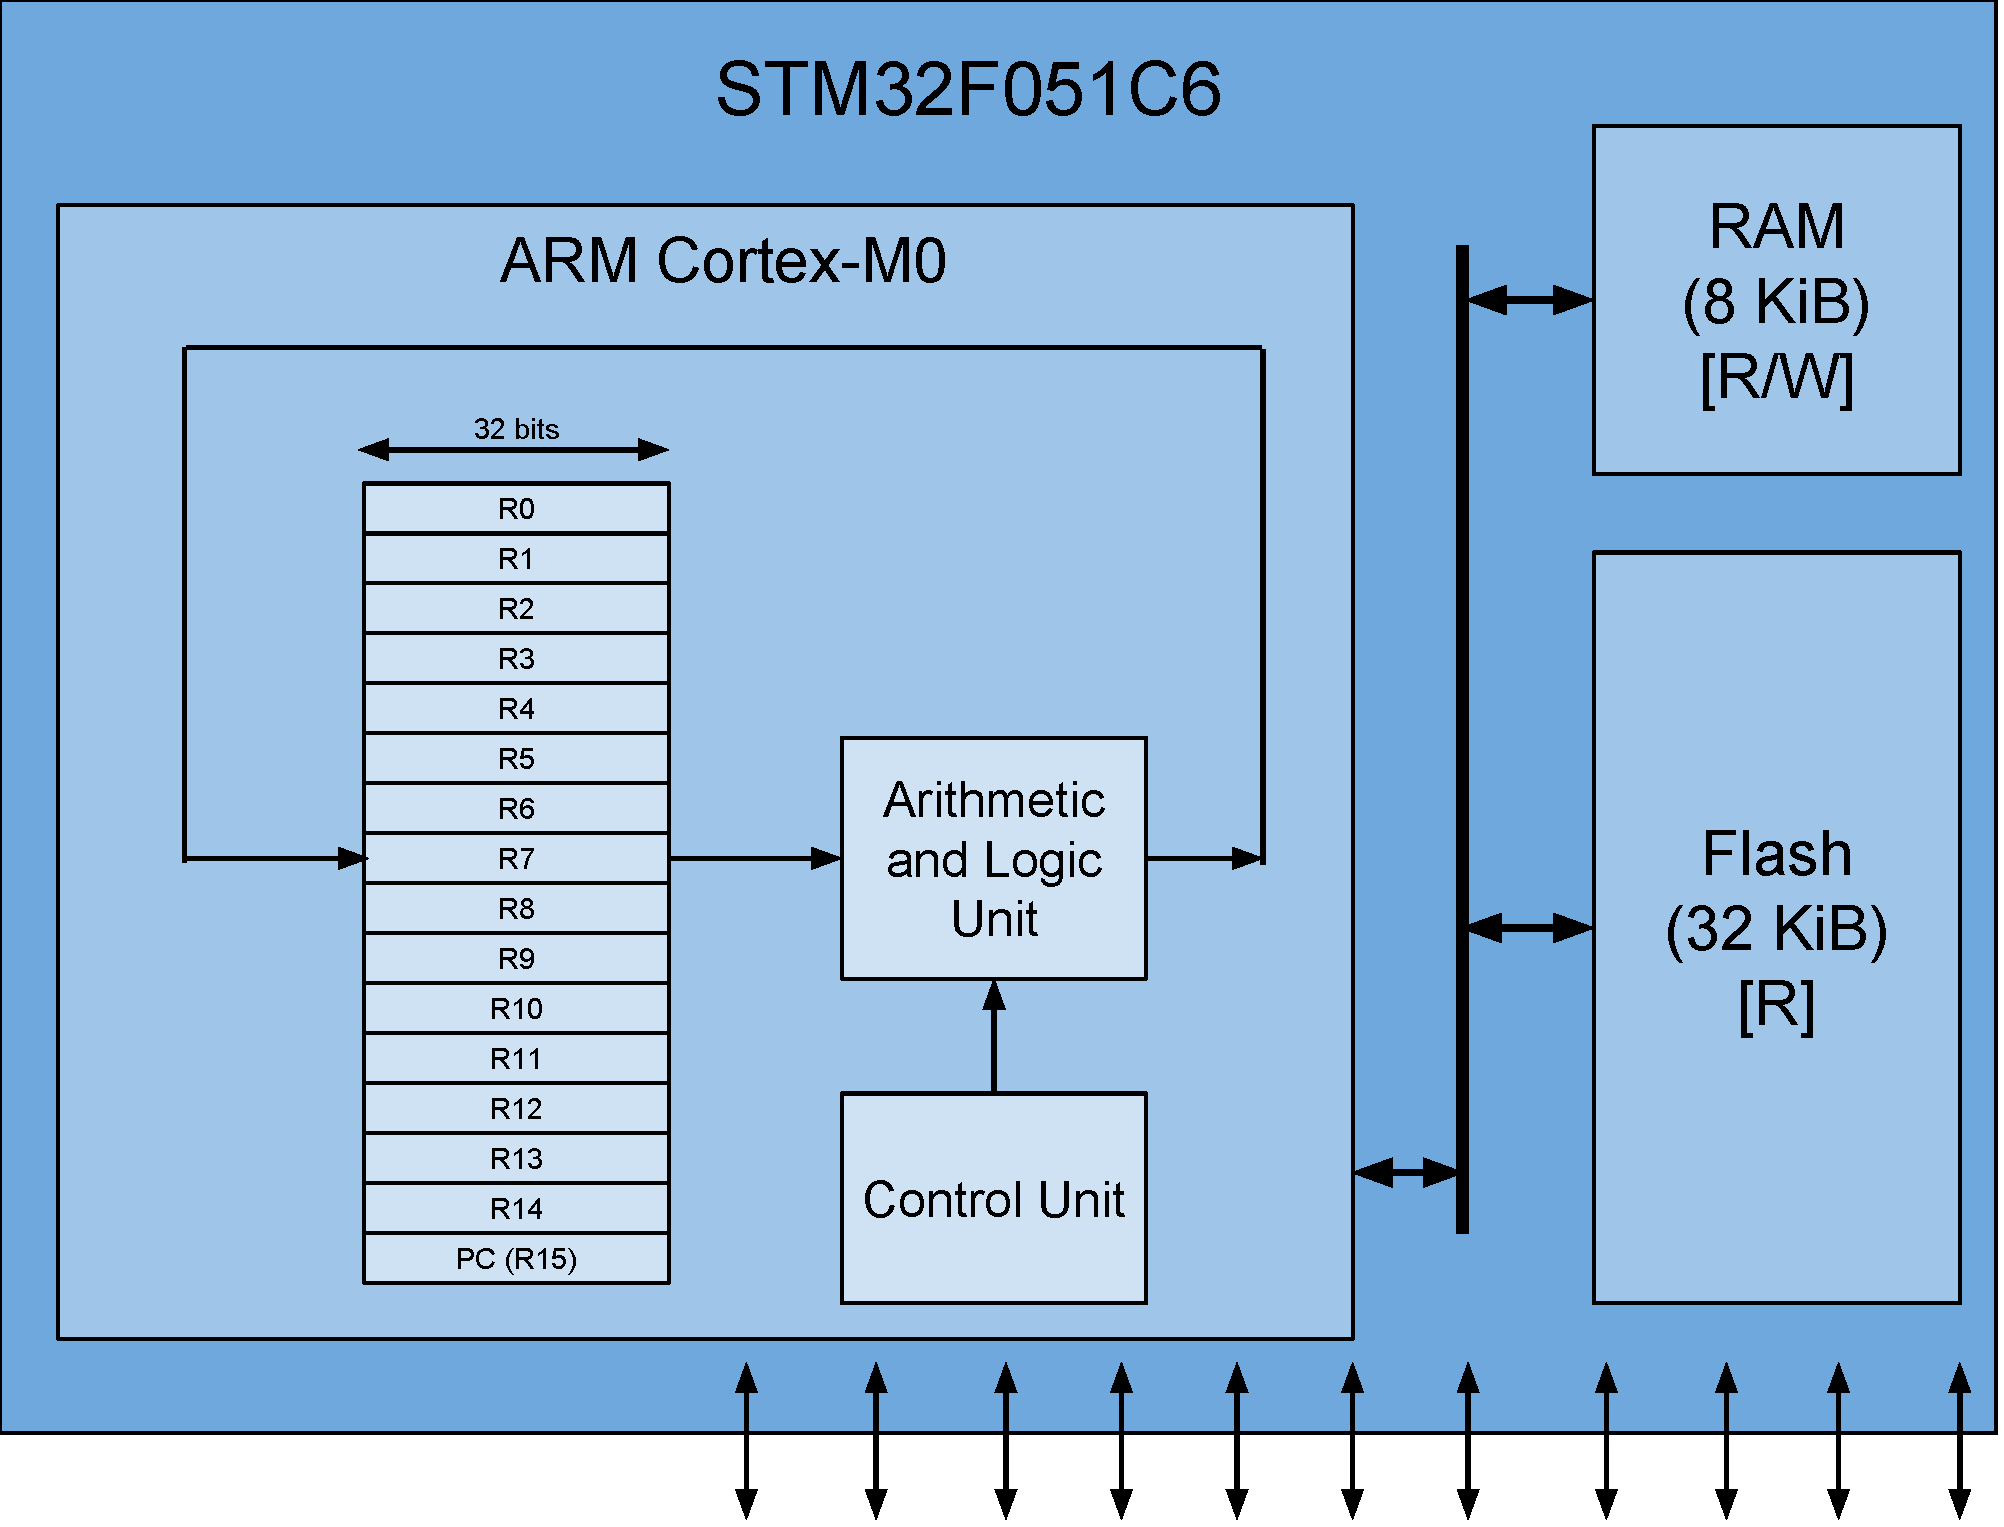
\includegraphics[width=0.9\textwidth]{./week1/programmers_model_v1.pdf}
  \caption{A view of the internals of the STM32F051 with the ARM Cortex-M0 expanded}
  \label{fig:prog_mod_v1}
\end{figure}
A programmer's model is a representation of the inner workings of the CPU with sufficient detail to allows us to develop code for the CPU, but no unnecessary detail. The expanded view of the CPU which will now be discussed can be seen in \autoref{fig:prog_mod_v1}. This simple model of a CPU is a set of CPU registers, an Arithmetic and Logic Unit (ALU) and a control Unit. The CPU registers are blocks of storage each 32 bits wide which the CPU has the ability to operate on. Only data which is inside a CPU register can be operated on by the CPU. The ARM Cortex-M0 has 16 such registers. 

The ALU is that which performs the operations on the registers. It can take data from registers as inputs, do very basic processing and store the result in CPU registers. 

The control unit manages execution by telling the ALU what to do. Together, the registers, ALU and control are able to execute instructions. 
Examples of instructions which the CPU is able to execute:
\begin{enumerate}
  \item adding the contents of R0 and R1 and storing the result in R6
  \item copying the contents of R3 into R0
  \item doing a logical XOR of the contents of R3 with the contents of R4 and storing the result in R3
  \item moving the number 42 into R5
\end{enumerate}


\section{CPU Architecture}
This section will explore some CPU architectures and compare them to the architecture of the Cortex-M0.

The Cortex-M0 makes use of a Von Neumann architecture. This means that there is a single bus which connects all of the parts (such as CPU, RAM, flash)  inside the microcontroller. The implication of this is that the CPU cannot fetch an instruction from flash at the same time as it moves data in or out of RAM. This limitation allows for a much simpler architecture, but at the expense of performance. 

Other microcontrollers (even others in the Cortex-M series like the Cortex-M3) follow a Harvard architecture, meaning that there are separate buses used for fetching instructions and moving data around. This allows faster execution as instructions can be fetched at the same time as data is loaded or stored. However, it necessitates greater complexity and more transistors. \\

It's been said that the ARM Cortex-M0 is a 32-bit processor. For comparison, the procesor which we used in this course previously (MC9S08GT16A) was an 8-bit processor. Your personal computer probably has a 64-bit CPU. 16-bit CPUs are also quite common. So what exactly does it mean when we say that the processor is 32-bits? Essentially, the number of bits which a processor is said to be referes to the size of the data bus. In other words: the amount of data which the processor is able to move around internally or perform arithmetic and logic operations on. Hence, with a 32-bit processor, we can move 32 bits of data from one spot in memory to another in just once instruction. If you had a 8-bit processor, it would cost 4 instructions to move 32 bits of data around.  

\subsection{Three stage pipeline}
Before discussing how loads or stores are done, the processor pipeline should be understood as it affects how the load instruction works. 
The ARM Cortex-M0 implements a three stage pipeline. This means that an instruction is broken up into three parts, and executed over the course of three clock cycles. The parts are:
\begin{itemize}
\item \textbf{fetch:} the instruction which the program counter points to is pulled into the CPU.
\item \textbf{decode:} the CPU control unit "looks" at the 16 bits which represent the instruction, and figures out what action it must take.
\item \textbf{execute:} the CPU runs the instruction, causing data to be modified.
\end{itemize}
The fact that the CPU is pipelined means that different instructions can be going through different phases \emph{at the same time}. In other words, one instruction can be being fetched while another is being decoded while another is being executed. 
As an example, assume we have three instructions which we want to execute, instruction A, instruction B and instruction C. The three instructions being run through the pipeline is shown graphically in \autoref{fig:pipeline}. It's critical to note how the program counter is always pointing to the instruction being \emph{fetched}. This makes sense as the job of the program counter after all is to facilitate keeping track of which instruction must be fetched. For this reason, when an instruction is being executed, the PC is actually pointing to two instructions (four bytes) further ahead in memory, and \emph{not} at the address of the instruction in execution. Hence, when an instruction in execution uses the PC, the value which will be used is the address of the instruction plus four.
\begin{figure}
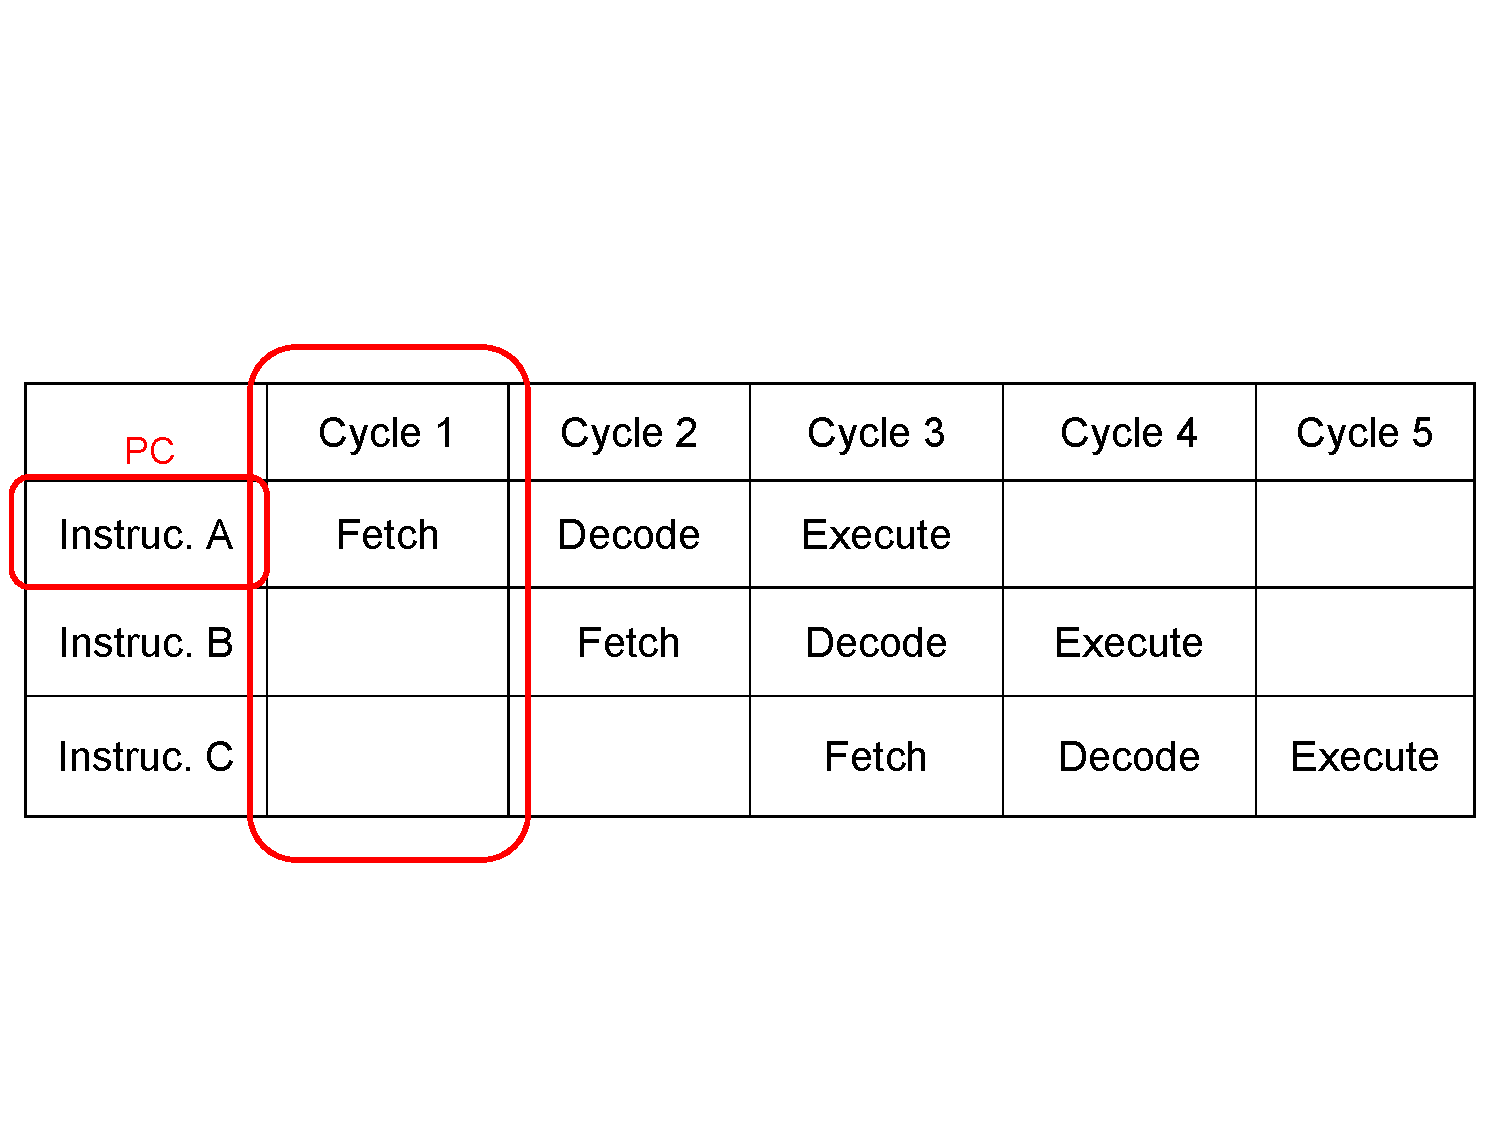
\includegraphics[page=1, clip=true, trim=1mm 40mm 1mm 57mm, width=\textwidth]{./week2/pipeline}
\includegraphics[page=2, clip=true, trim=1mm 40mm 1mm 57mm, width=\textwidth]{./week2/pipeline}
\includegraphics[page=3, clip=true, trim=1mm 40mm 1mm 57mm, width=\textwidth]{./week2/pipeline}
\caption{Showing three instructions being run through a three stage pipeline, as well as where the PC is pointing every cycle}
\label{fig:pipeline}
\end{figure}

\chapter{Memory Model}
We will now beging to expand on some of the block is \autoref{fig:prog_mod_v0}. Before starting to explore how the CPU works, it's useful to have an understanding of how memory is laid out. We will start looking at the flash and RAM blocks. Together with another block called perihperals (which we will explore later), these blocks make up memory. 
It's important to note that this memory is located \emph{outside} of the CPU, but still inside the microcontroller IC.

The memory of a device can be though of as a very long row of post boxes along a street. 
Each post box has an address, and each post box can have data put into it or taken out. The amount of data that each post box can hold is 8 bits, or one byte. Therefore, each memory address is said to address one byte. 
The address of each post box is 32 bits long, meaning that addresses range from 0 (0x00000000) to just over 4.3 billion (0xFFFFFFFF). In actual fact, the \emph{vast} majority of these addresses do not have a post box at them. These addresses are said to be unimplemented. 
Only very small sections of this address space are implemented and can actually be read from or written to.
Flash and RAM are contiguous blocks of memory, with a start address and an end address. A simplified memory map of the STM32F051 is shown in \autoref{fig:memory_map}. From this, we can see that if we want to use changeable variables in our programs, the variables should be located at addresses between 0x2000 0000 and 0x2000 1FFF. If we want to load code onto the micro which should not be lost when the device loses power, the code should be loaded into the non-volatile memory, flash, which has addresses between 0x0800 0000 and 0x0800 7FFF.
If we want the ability to modify data during the execution of our program, the data should be placed in the read/write section of memory, RAM. 

\begin{figure}
  \centering
  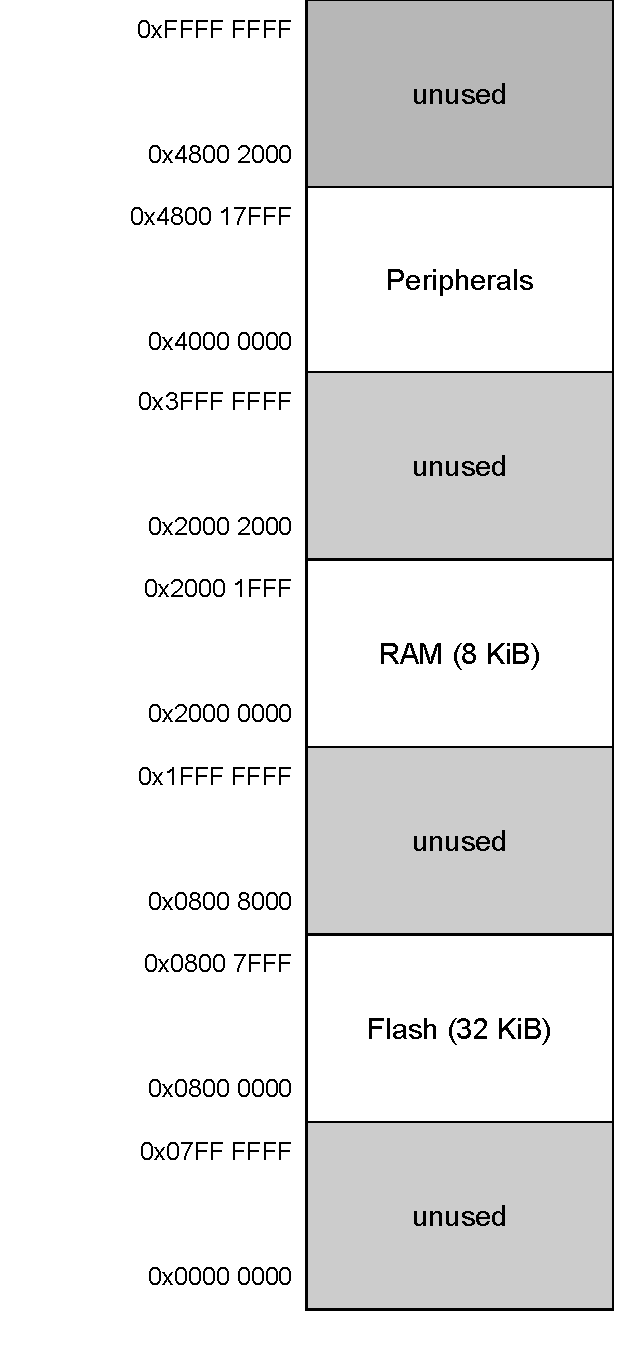
\includegraphics[width=0.6\textwidth]{./week1/memory_model_v0.pdf}
  \caption{Simplified STM32F051C6 memory map. Note how all addresses are 32 bits. The blocks are very much not to scale. Source: datasheet, Figure 9}
  \label{fig:memory_map}
\end{figure}

\section{Data Types and Endianness}
Very often we will need to work with clumps of data which are larger than 1 byte. ARM defines datatypes for a 32 bit CPU as follows:
\begin{itemize}
  \item byte: 8 bits
  \item halfword: 16 bits
  \item word: 32 bits
  \item doubleword: 64 bits
\end{itemize}
Each memory address only addresses one byte of memory, so how can something like a word (four bytes) be stored in memory? 
Obviously, the four bytes have to come after each other to form a four byte block, or word.
However, it is not obvious which order they should come in. For example, consider the case of wanting to store the word 0xAABBCCDD in address 0. The two possible ways of doing it are shown in \autoref{tab:endianness}. It doesn't really matter which one of these schemes is used - they each have their pros and cons and different processors use different methods. It is important to know which one our processor has chosen to use. Our processor uses little endian. A more abstract view of how data is stored in our processor is given in \autoref{fig:little_end_prog_man}
\newpage
\begin{table}
\centering
\begin{tabu}{cc}
    \multicolumn{2}{c}{\textbf{Little Endian}}\\
    \hline
    Address & Data \\
      \hline
      3 & 0xAA \\
      2 & 0xBB \\
      1 & 0xCC \\
      0 & 0xDD \\
\end{tabu}
\qquad
\begin{tabu}{cc}
    \multicolumn{2}{c}{\textbf{Big Endian}}\\
    \hline
    Address & Data \\
      \hline
      3 & 0xDD \\
      2 & 0xCC \\
      1 & 0xBB \\
      0 & 0xAA \\
\end{tabu}
\caption{Layouts of the word 0xAABBCCDD in memory at effective address 0, according to little or big endian format}
\label{tab:endianness}
\end{table}

\begin{figure}
  \centering
  \includegraphics[width=0.8\textwidth, page=21, clip=true, trim=160px 285px 160px 427px]{./stm32f0xx_programming_manual.pdf} % l b r t
  \caption{More abstract view of little endian layout. Source: Prog Man, page 28}
  \label{fig:little_end_prog_man}
\end{figure}

%\begin{overpic}[page=21, grid,unit=1px, tics=20, clip=true, trim=160px 285px 160px 427px]{./stm32f0xx_programming_manual.pdf}
%\end{overpic}


\chapter{Coding}

\section{Assembly}

In order to get the CPU to do some of what we've discussed above, it needs to have code loaded onto it to run. We write code in a language called assembly. Assembly is a human-readable language. A program is made up of a sequence of instruction; each instruction gets executed by the CPU. It's quite easy to see what each instruction does by reading the program.  The complete instruction set is located in the Programming Manual. You must be familiar with this document! Examples of instruction which carry out the tasks listed above are:
\begin{enumerate}
  \item \texttt{ADDS R6, R0, R1}
  \item \texttt{MOV R0, R3}
  \item \texttt{EORS R3, R3, R4}
  \item \texttt{MOVS R5, \#42}
\end{enumerate}
The CPU does not have the ability to understand our nice English words like \textit{ADD} or \textit{MOV}. The CPU only has the ability to understand binary data. Assembly code must be compiled to machine code. A machine code instruction is a binary string, 16 bits long consisting of the operation code (opcode) and the data which it must operate on (operand).
For example, assume that we wanted to ascertain the machine code representation of the instruction \texttt{ADDS R6, R0, R1}. An extact from the ARMv6-M Architecture Reference Manual is shown in \autoref{fig:adds_encoding} where Rd is the destination register and Rm and Rn are the source registers of the add. It can easily be seen that the instruction would compile to\texttt{ 0001100 001 000 110 = 0x1846}.
\begin{figure}
\centering
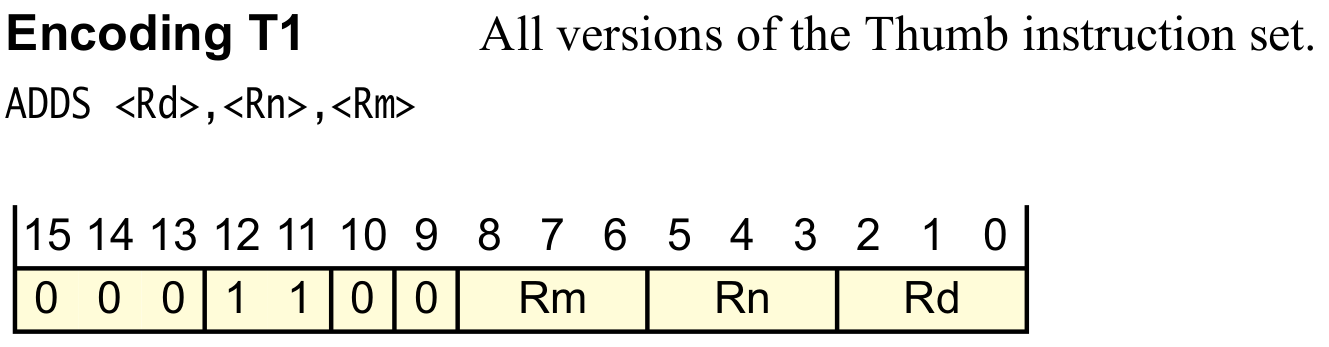
\includegraphics[width=0.7\textwidth]{./week1/adds_encoding}
\caption{An encoding of the ADDS instruction}
\label{fig:adds_encoding}
\end{figure}
The opcodes for each instruction are detailed in the ARMv6-M Architecture Reference Manual.
All of the instructions in the program are 16 bits long and are stored sequentially after one another in flash memory. 


\subsection{Instruction Sets}
An instruction set is the collection of all of the instructions which a processor can execute. 
The ARM Cortex-M0 uses the ARMv6-M architecture and this architecture supports the Thumb instruction set (as opposed to Thumb-2 or ARM). 
Thumb contains about \emph{XXX} instructions, each of which is 16 bits long. \\

Higher end ARM processors such as the Cortex-M3 or Cortex-M4 support the ARMv7-M architecture which allows multiple instruction sets to be supported by the processor. 
The ability to support multiple instruction sets requires \emph{interworking}. Interworking is the ability to specify to the CPU which instruction set to use. 
While our ARM Cortex-M0 only supports the Thumb instruction set, there is no need for interworking, yet the cabability has still been incorperated into the architecture to allow for compatability to other processors. 
This means that although our processor only supports one instruction set (Thumb), we have to explicity tell it that we are using that instruction set. 


\section{Linking}
Once our assembly code has been written and compiled to machine code, the computer which loads the code onto the micro has to be told what addresses to place the code at. The code should be placed starting at the beginning of flash.

\subsection{Executing Code}
The PC always points to the instruction which is about to be fetched. Hence, when your micro boots up, before it has executed anything, the PC will point to the first instruction to be fetched/decoded/executed.
By "point to" we mean that it holds the address of the instruction. 

As each instruction in the ARM Cortex-M0 instruction set it 16 bits (aka: half a word) long, ARM have implemented a rule that all instructions must be half word alligned. In other words, the address of the instruction must be divisible by 2 bytes. Legal addresses for instructions are hence, 0x02, 0x04, 0x06, 0x08 ... etc. 
This means that the least significant bit (bit 0) of the PC register is unused in specifcying the address of an instruction. 
Hence, it has been assigned another use. Specifically, to indicate the instruction set which is being executed. 



\chapter{Loading and Storing}

Loading is the process of getting data from somewhere in the memory space into the CPU registers so that it can be used in processing. Storing is the process of getting data which is in the CPU registers into memory. Remember that seeing as flash is read-only memory, we cannot store data to flash address, but we can store to RAM.

The general format for a load is that a destination register, a register containing a base address, and an offset are supplied. An effective address is then calculated as the base address plus the offset. The contents of memory at the effective address are then copied from memory into the destination CPU register. When we do this we are treating a register as a \emph{pointer}. When we regard the contents of a register as a memory address and use that register to access data in memory we are dereferencing a pointer: accessing the data pointed to by a pointer. This is an important concept!

A store operation is very similar. Again, a register containing a base address and an offset are supplied, but this time it is a source register not a destination register which is supplied. Again, and effective address of base plus offset is calculated. The contents of the source register is copied into the effective address. 

Note that most of the load/store operations which we will be doing are 32-bit (word) load or stores. This is because the CPU registers are 32 bits. So far we have only spoken of a single effective address. As you know, each address can only hold 8 bits. Hence, in order to load or store 32 bits, four sequential addresses are used. The effective address specifies the \emph{lowest} in the sequence of the addresses. For example, if we wanted to store the contents of R0 in 0x20000000, the word would be placed into the address range 0x20000000, 0x200000001, 0x20000002 and 0x20000003. Remember that our processor uses little endian format, so the LSB is placed at 0x20000000 and the MSB at 0x20000003.

We will now explore some implementations of loading and storing.

\section{Immediate Offset Loading}
In this format, the base address is supplied in one of high CPU registers (R0 - R7), and the offset is supplied as an immediate number. 
The instruction format for loading data into a register is
\begin{lstlisting}[fontadjust=true,frame=trBL]
LDR Rt, [Rn, #imm]
\end{lstlisting}
where \texttt{Rt} is the target register for the load, \texttt{Rn} contains the base address and \texttt{\#imm} is the offset from the base address.

The way that this instruction works is that it calculates an \emph{effective address} which is equal to the contents of the base address register plus whatever number is supplied as an immediate operand.
There is, however, a slight complexity in how the offset is dealt with.

\subsection{Offset restrictions}
\label{sec:load-store-restrictions}
Remember that all instructions are limited to 16 bits. The format of the LDR instruction in machine code is shown in \autoref{fig:ldr}. We can see that after 5 bits of opcode and $2 \times 3 = 6$ bits of register specifications, we are only left with 5 bits of offset. Normally, these 5 bits would only allow us to provide an offset of $2^5 - 1 = 31$ bytes. This is not very much! In order to extend the range of the 5 offset bits, the actual offset used is equal to the 5 bit immediate number multiplied by four. This multiplication by four is the same as appending two zeros to the end of the binary value, which you can see is being done in \autoref{fig:ldr}. This means that the amount which we are able to offset a base address by is now $(2^5 - 1) \times 4 = 124$, which is significantly more useful. However, seeing as we are multiplying to immediate number by four to get the actual offset, the implication is that all offsets \emph{must} be a multiple of four. 
The compiler automatically takes care of dividing whatever offset we supply in our assembly instruction by four in order to get it to fit into the 5 bit immediate number, and the CPU then multiplies the immediate number by four to get the offset.

For example: if we wanted an offset of 12, the immediate number which would be placed in the instruction by the compiler would be 3.

\begin{figure}
\centering
\includegraphics[page=139, clip=true, trim=35mm 157mm 55mm 40mm, width=0.85\textwidth]{./DDI0419C_arm_architecture_v6m_reference_manual}
\caption{Machine Code representation of LDR instruction. Source: ARMv6-M Architecture Reference Manual}
\label{fig:ldr}
\end{figure}

\section{Program Counter Relative Loading}
There is another format of the LDR instruction which takes the Program Counter as a base register, and allows for an 8-bit immediate offset. If you wish to load data from flash into a CPU register, it makes sense to use the PC as a base register due to the fact that the PC is already initialised to be pointing to an address in flash. Specifically, it is pointing to the instruction which is being fetched (not executed - remember the three stage pipeline!). The format of the LDR instruction for PC relative loading can either be specified in the same was as the general LDR instruction, or it can have a label provided as an operand, as follows:
\begin{lstlisting}[fontadjust=true,frame=trBL]
LDR Rt, [PC, #imm]
LDR Rt, <label>
\end{lstlisting}
If one supplies a label as an operand, all that the compiler does is calculate the correct immediate offset value to insert, and compiles the instruction as if it were in the first format. It's important to note that these instructions are exactly equivalent: all that using a label does is cause the compiler to do the hard work of calculating the correct offset so you don't have to. It would really be a lot of hard work; every time you changed something in the structure of your program which caused instructions to be moved to different memory addresses (like writing a new line of code!) you'd potentially have to re-calculate your offsets. The ability to use labels is one of the most useful features of the compiler.


\section{Register Offset Loading}
So far all offsets have been supplied as immediate numbers to the load instructions. However, there is another format of the load instruction called a register-offset load. Here, the offset is contained in another register. This is useful as the offset can be set at run-time by modifying the contents of a register, rather than at compile time. In this case, the effective address is calculated as the contents of the base register (\texttt{Rn}) plus the contents of the offset register (\texttt{Rm}). 
\begin{lstlisting}[fontadjust=true,frame=trBL]
LDR Rt, [Rn, Rm]
\end{lstlisting}

\section{Storing}
The storing commands are so similar to the loading that they will barely be discussed. One difference is that there is no PC-relative store, as there would be no point trying to store data to read-only memory. The store instruction takes moves the contents of a source register, \texttt{Rt}, and places it at the effective memory address equal to the base address, \texttt{Rn}, plus an offset either supplied as a 5-bit immediate number, \texttt{\#imm5}, or in an offset register, \texttt{Rm}.

\begin{lstlisting}[fontadjust=true,frame=trBL]
STR Rt, [Rn, #imm5]
STR Rt, [Rn, Rm]
\end{lstlisting}

\section{Accessing of Datatypes Other Than Words}
So far we have only loaded or stored words. While it is useful to be able to move an entire 32 bits of data around at once we will sometimes only want to move bytes of half-words around. There are instructions which allow us to do this. There is a version of the \texttt{LDR} instruction which loads only 1 byte: \texttt{LDRB}. Similarly, there is a version which loads 2 bytes or half a word: \texttt{LDRH}. 


\end{document}
